\documentclass{article}
\usepackage[utf8]{inputenc}
\usepackage{graphicx}
\usepackage{subcaption}

\title{Challenges in chaotic time series forecasting}
\author{Maximilian Hornung}

\begin{document}
\maketitle

\begin{abstract}
  Predicting the future development of time series is of interest in different
  areas of computational biology. The time series in biological models exhibit
  challenging characteristics such as chaotic or stochastic behavior. In this
  report, time series prediction is done on different kind of biological time
  series using deep neural networks. In our evaluation, we identify challenges
  and limitations of this approach, and compare different architectures of
  deep neural networks with regard to their performance.
\end{abstract}

\section{Introduction}

In various kind of diseases, it is important to choose the correct treatment at
the current time point. Since the human body is too complex to be described
directly using mathematics, special features are modeled with mathematical
systems such as the Mackey-Glass equations for respiratory and hematopoietic
diseases \cite{mackey1977}. These models make use of available data about
previous information in order to reduce the uncertainty under which a decision
is done. This is especially important when the consequences of a decision are
severe, for example the decision of breast cancer treatment after radiation.
This particular problem can be addressed by using a stochastic differential
equation, as done by Oroji \textit{et al} \cite{oroji2016}.

In different kinds of biological models, chaotic behavior is observed. The
Mackey-Glass equations possess chaotic behavior for certain choices of their
parameters, as shown by Fischer \cite{farmer1982}. That means that even small
measurement errors of the initial state lead to exponentially increasing
errors of the time series prediction. Because of that, it is important
that the time series prediction should be as robust as possible against noise.

This gets imporant in particular because another characterstic of dealing with
biological data is the presence of noise. In
this report, we show that different kinds of noise assumptions can impact the
results of time series prediction. We evaluate all our investigated problems
with regard to the popular $i.i.d.$ random noise as well as noise from a
discretized Wiener process, i.e. memorizing random
noise. Since mathematical models of biological systems can not describe their
characteristics perfect and error-free, it is assumed that the latter type of
noise is more realistic. But unfortunately this kind of noise increases the
difficulty of time series prediction, even for simple mathematical functions,
as seen in Section~\ref{sec:sine}.

The remaining report is structured as follows. First, we perform proper time
series prediction on the sinus function and show how different noise models
impact the prediction ability of our network models. After that, we show how
different levels of chaos impact the possibility to forecast the development
of time series at the example of the \emph{Mackey Glass} time series. We show
how the stochasticity of noise impactss the possibility to predict deterministic
chaotic time series at the example of the \emph{Mackey Glass} time series. Last
but not least, we report fundamental limitations of neural networks to
approximate stochastic time series at the example of biological oscillators.

\section{Methods}

In our analysis, we use three different architectures and neural networks and
optimize their hyperparameters for the respective use case. Since Hornik
\textit{et al.} have shown that feedforward neural networks are universal
function approximators \cite{hornik1989}, we evaluate this architecture with
varying number of hidden nodes.

After that, we investigate the strength of
improvement of using a recurrent neural network. This type of neural network has
already been applied to time series prediction \cite{connor1994}, but suffers
from the vanishing gradient problem when capturing long-term dependencies in a
sequence. Because of that, we decide to evaluate only the Long Short-Term Memory
(\textbf{LSTM})
network architecture \cite{hochreiter1997}, which was successfully applied in
various time series prediction tasks like anomaly detection \cite{malhotra2015},
stock price \cite{fischer2018} and protein disorder prediction
\cite{hanson2016}.

In the last years, convolutional neural networks (\textbf{CNN}s) have improved
the results in image classification \cite{krizhevsky2012} and other computer
vision tasks. A \textbf{CNN} learns features from the data in a hierarchical
way, for example combining pixels to edges, edges to more complex forms etc.
until a high-level classification can be done. The large success in computer
vision has inspired researchears in time series prediction to also apply
\textbf{CNN}s \cite{cui2016, borovykh2017}, so we also evaluate this
architecture in our analysis. The same way as images are composed of
hierarchical features (e.g. a face consisting of eyes, that consist of
certain edges etc.) we assume that similar hierarchies of features can be found
in time series data.

All implementation is done using the \texttt{Python} programming language in
version $3.6.7$. The time series data is created and loaded in the
\texttt{numpy} framework in version $1.16.1$. In order to train the neural
networks both fast and elegant, we use the \texttt{keras} (version $2.2.4$)
with the
\texttt{tensorflow} backend in version $1.13.1$.
The reason for this choice is the tight
integration between \texttt{keras} and \texttt{numpy} that simplifies and
increases the speed of our software development. Before running the experiments,
the random number generator of \texttt{numpy} is set to the seed $0$ to ensure
reproducibility of our results.

\section{Evaluation}
\subsection{Time series forecasting of periodic functions}
\label{sec:sine}
In the first part of the analysis, we analyze the capability of different neural
network architectures to perform time series prediction on the periodic sinus
function. This task can be considered simple, because the different parts of the
sine wave occur multiple times in the data, i.e. the function is periodic.
It is therefore interesting how
robust the network architectures are with regard to different kinds of noise.

In this section, we provide information about the last 10 time sequence points
to the network and want to predict the next point, as given in
Equation~\ref{equ:sine}. That is, we want to estimate $x(t)$ with a function
$F(x(t), x(t-1), \cdots, x(t-9))$ that is computed using a neural network.

\begin{equation}
  \hat{x} (t + 1) \approx F(x(t), x(t-1), \cdots, x(t-9))
  \label{equ:sine}
\end{equation}

We consider two different types of noise. First, we consider $i.i.d.$ gaussian
noise which is added to the underlying function $f(t)$
as seen in Equation~\ref{equ:iid_noise}. The other type of noise is a
discretized Wiener process, i.e. a memorizing type of noise that is shown in
Equation~\ref{equ:wiener}.
For more details about Wiener processes, refer to Schilling
\textit{et al} \cite{schilling2014}

\begin{equation}
  \forall t: \quad x(t) = f(t) + y, \quad y \sim \mathcal{N}(0, \sigma^2)
  \label{equ:iid_noise}
\end{equation}

\begin{equation}
  \forall t: x(t) = f(t) + y(t), \quad y(t) = y(t-1) + y \sim \mathcal{N}(0, \sigma^2), \quad y(0) = 0
  \label{equ:wiener}
\end{equation}
In Figure~\ref{fig:noise_impact}, we see that a densely connected neural network
with one hidden layer of 10 nodes is capable of performing the time series
prediction. Even if we apply $i.i.d.$ gaussian noise with standard
deviation $\sigma = 0.1$, the
network can still be trained to fit the data correctly. But if the noise is not
applied independently in each timestep, the convergence takes more time steps as
pointed out in Figure~\ref{fig:noise_loss_impact}. This effect is especially
strong for the \emph{LSTM} architecture, where even 100 epochs are not enough
for the validation loss to converge, compared to the other approaches that need
only 20 epochs.

Since the noise we apply on the data has a standard deviation $\sigma = 0.1$,
it is obvious that a perfect time series prediction is not be possible. We
expect that the minimum possible validation loss is as high as the variance
($\sigma^2$), and can reproduce that in all neural network architectures as
shown in Table~\ref{tab:noise_finals}. The validation loss of a perfect
neural network would therefore be $\sigma^2 = 0.01$, which is achieved by all
architectures for $i.i.d.$ noise. Only the LSTM architecture has worse
performance for the memorizing noise. We assume that this is due to the slower
learning of that architecture compared to the others when confronted with
memorizing noise. One possible reason for this observation is that the LSTM is
trying to capture temporal dependencies between points in the time series, which
is confused by the temporal dependencies induced by the memorizing noise.

\begin{table}
  \centering
  \begin{tabular}{l|c|c|c}
    Architecture & Noisefree data & $i.i.d.$ noise & memorizing noise \\
    \hline
    MLP          & 0.0021         & 0.0249         & 0.0174           \\
    LSTM         & 0.0021         & 0.0127         & 0.5554           \\
    CNN          & 0.0021         & 0.0136         & 0.0234           \\
  \end{tabular}
  \caption{Validation loss of different neural network architectures for
    time series prediction on the sinus function stated
    in RMSE.}
  \label{tab:noise_finals}
\end{table}

\begin{figure}
  \begin{subfigure}{.35\textwidth}
    \centering
    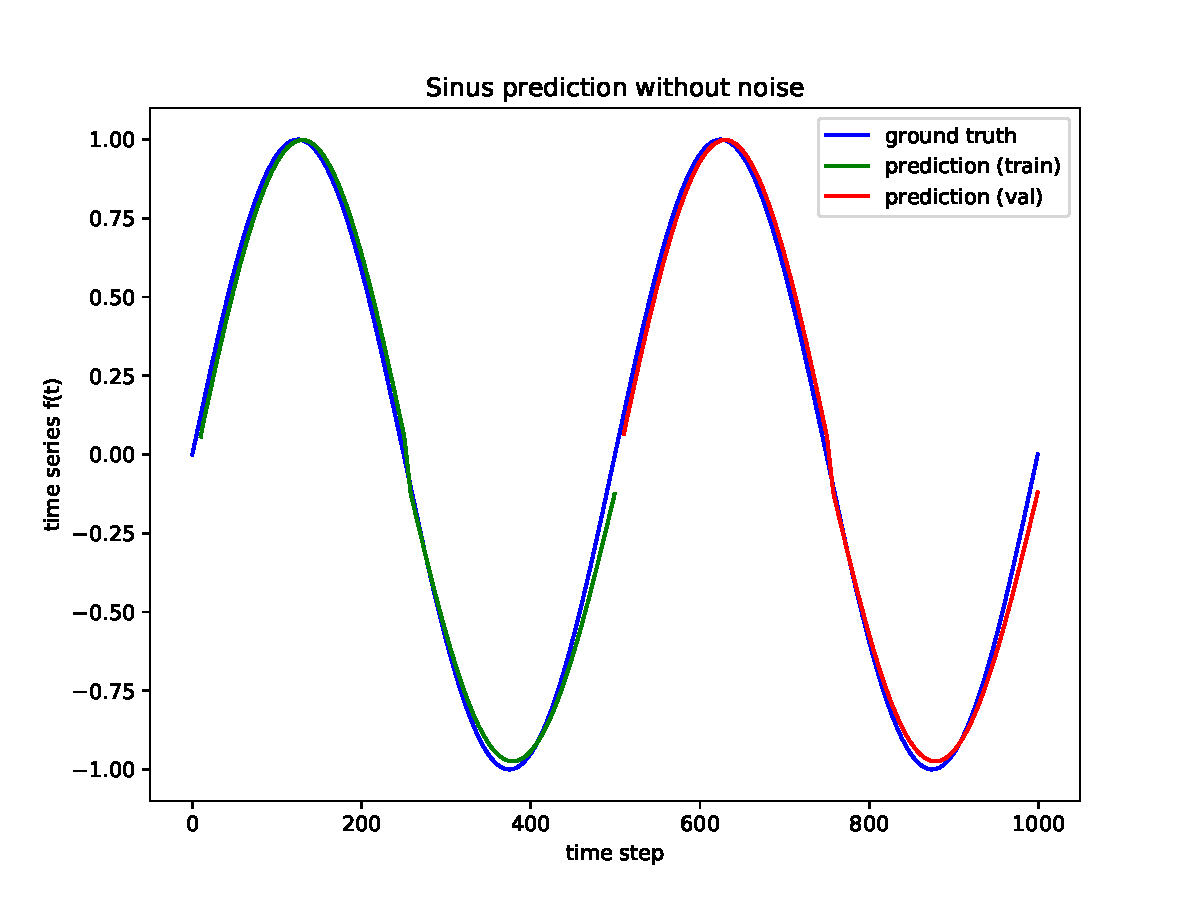
\includegraphics[width=\linewidth]{figures/plot_twolayer_noiseless.pdf}
  \end{subfigure}
  \hspace{-5mm}
  \begin{subfigure}{.35\textwidth}
    \centering
    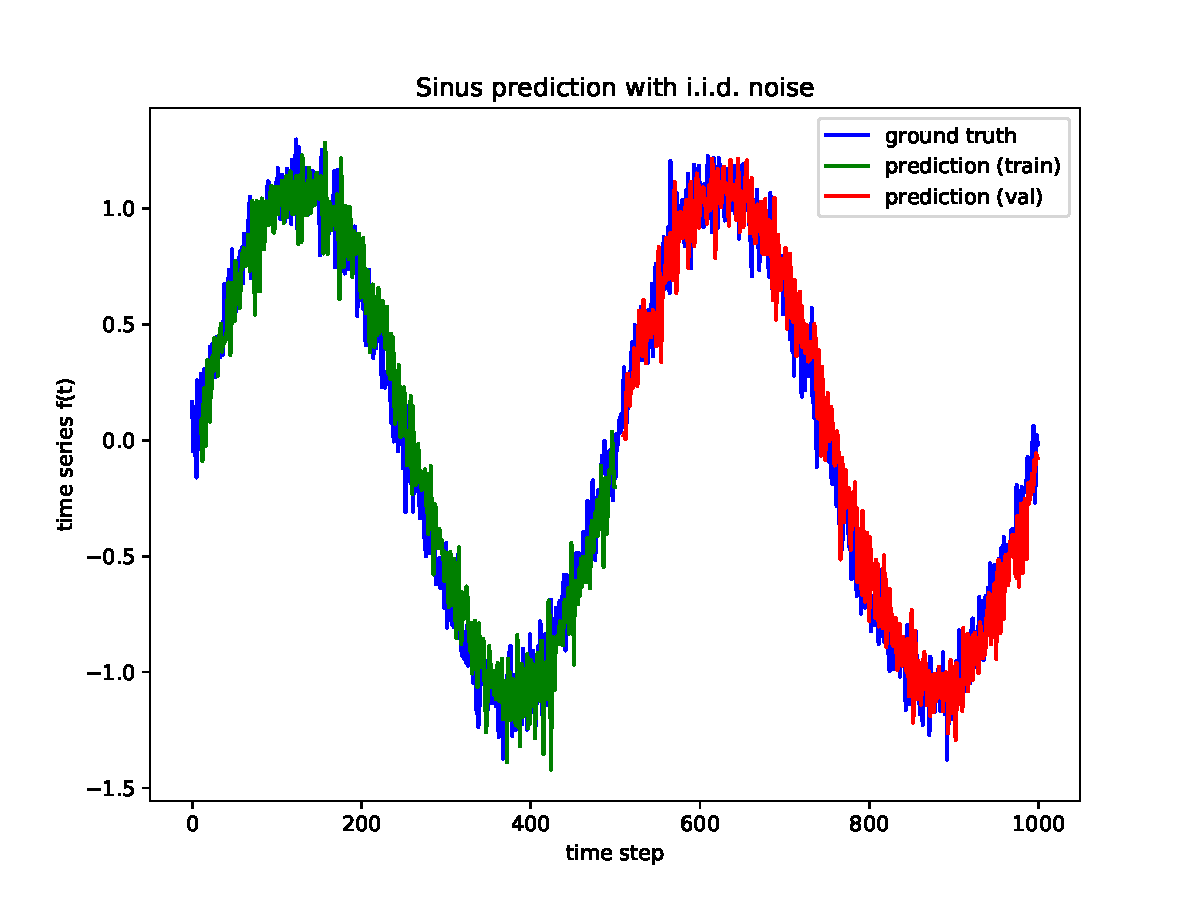
\includegraphics[width=\linewidth]{figures/plot_twolayer_iidnoise.pdf}
  \end{subfigure}
  \hspace{-5mm}
  \begin{subfigure}{.35\textwidth}
    \centering
    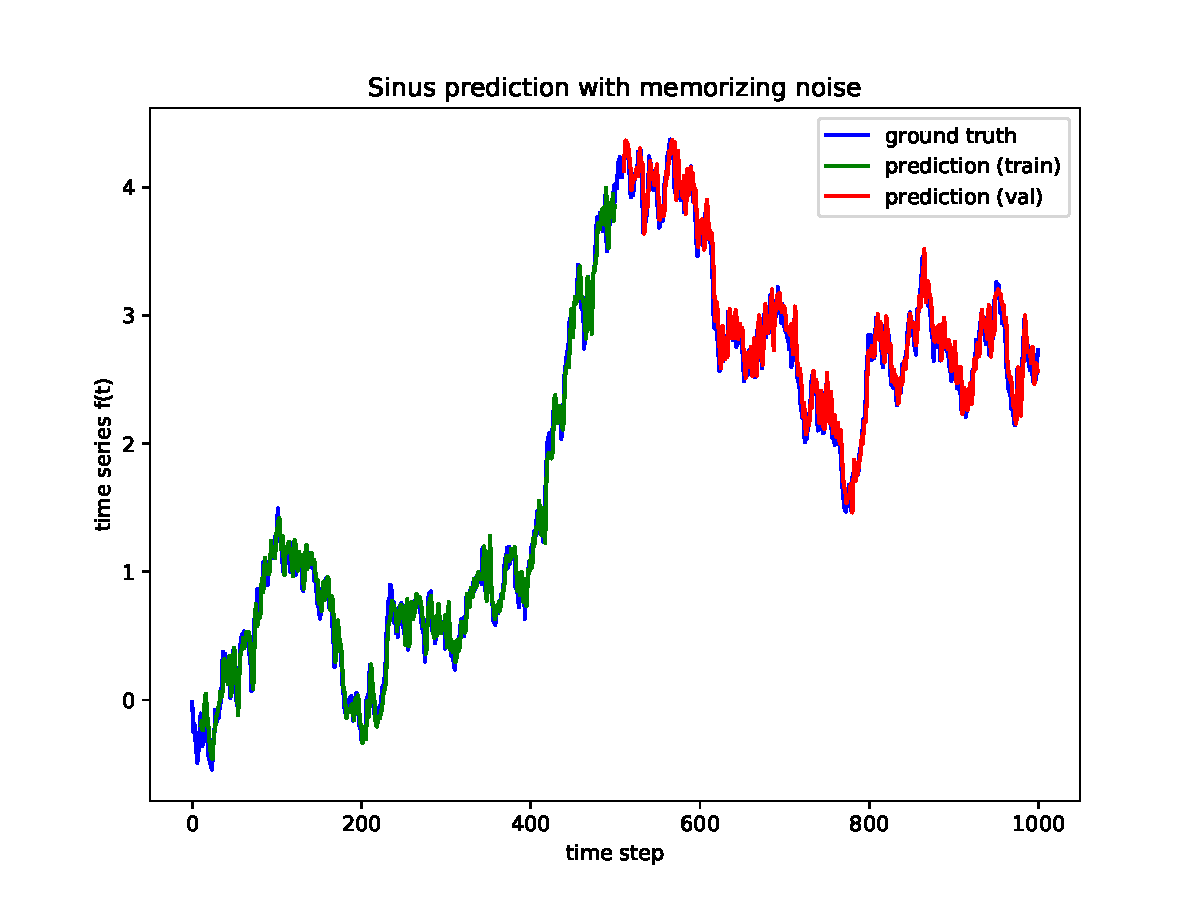
\includegraphics[width=\linewidth]{figures/plot_twolayer_memnoise.pdf}
  \end{subfigure}
  \caption{Impact of different kinds of noise on the time series prediction
    using a feedforward neural network with one hidden layer. Number of hidden
    units stays 10 in all simulations. The noise is normal distributed with $\sigma =
      0.1$.}
  \label{fig:noise_impact}
\end{figure}

\begin{figure}
  \center
  \begin{subfigure}{.35\textwidth}
    \centering
    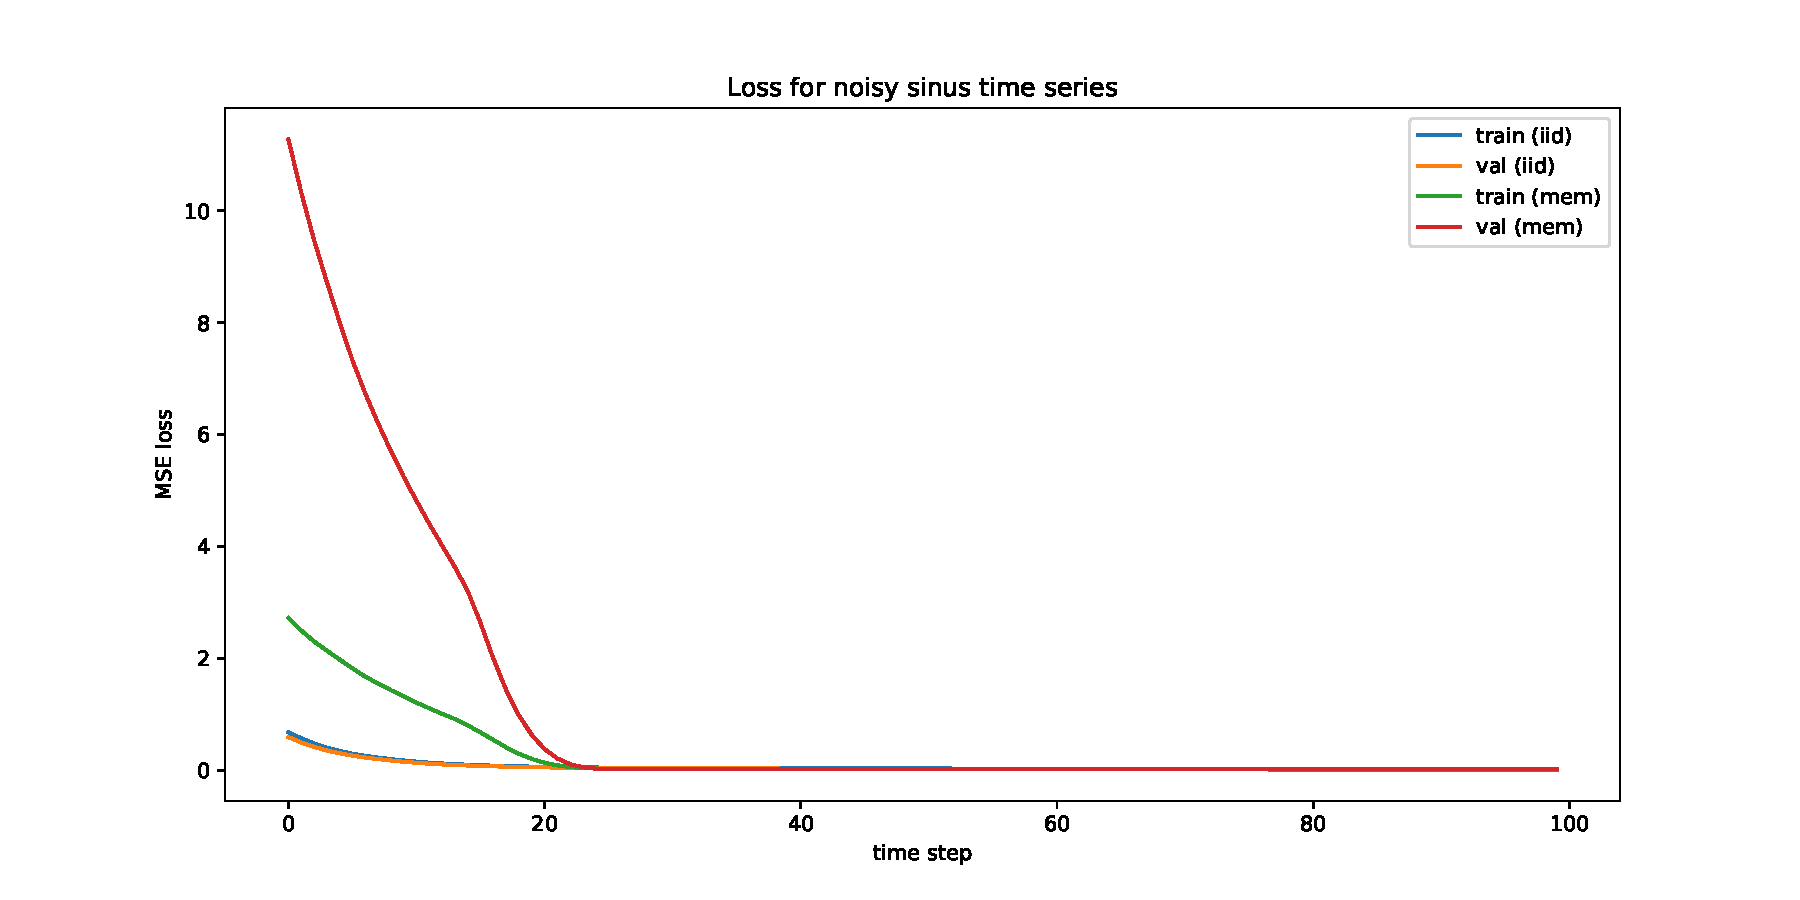
\includegraphics[width=\linewidth]{figures/plot_twolayer_losscompare.pdf}
  \end{subfigure}
  \hspace{-6mm}
  \begin{subfigure}{.35\textwidth}
    \centering
    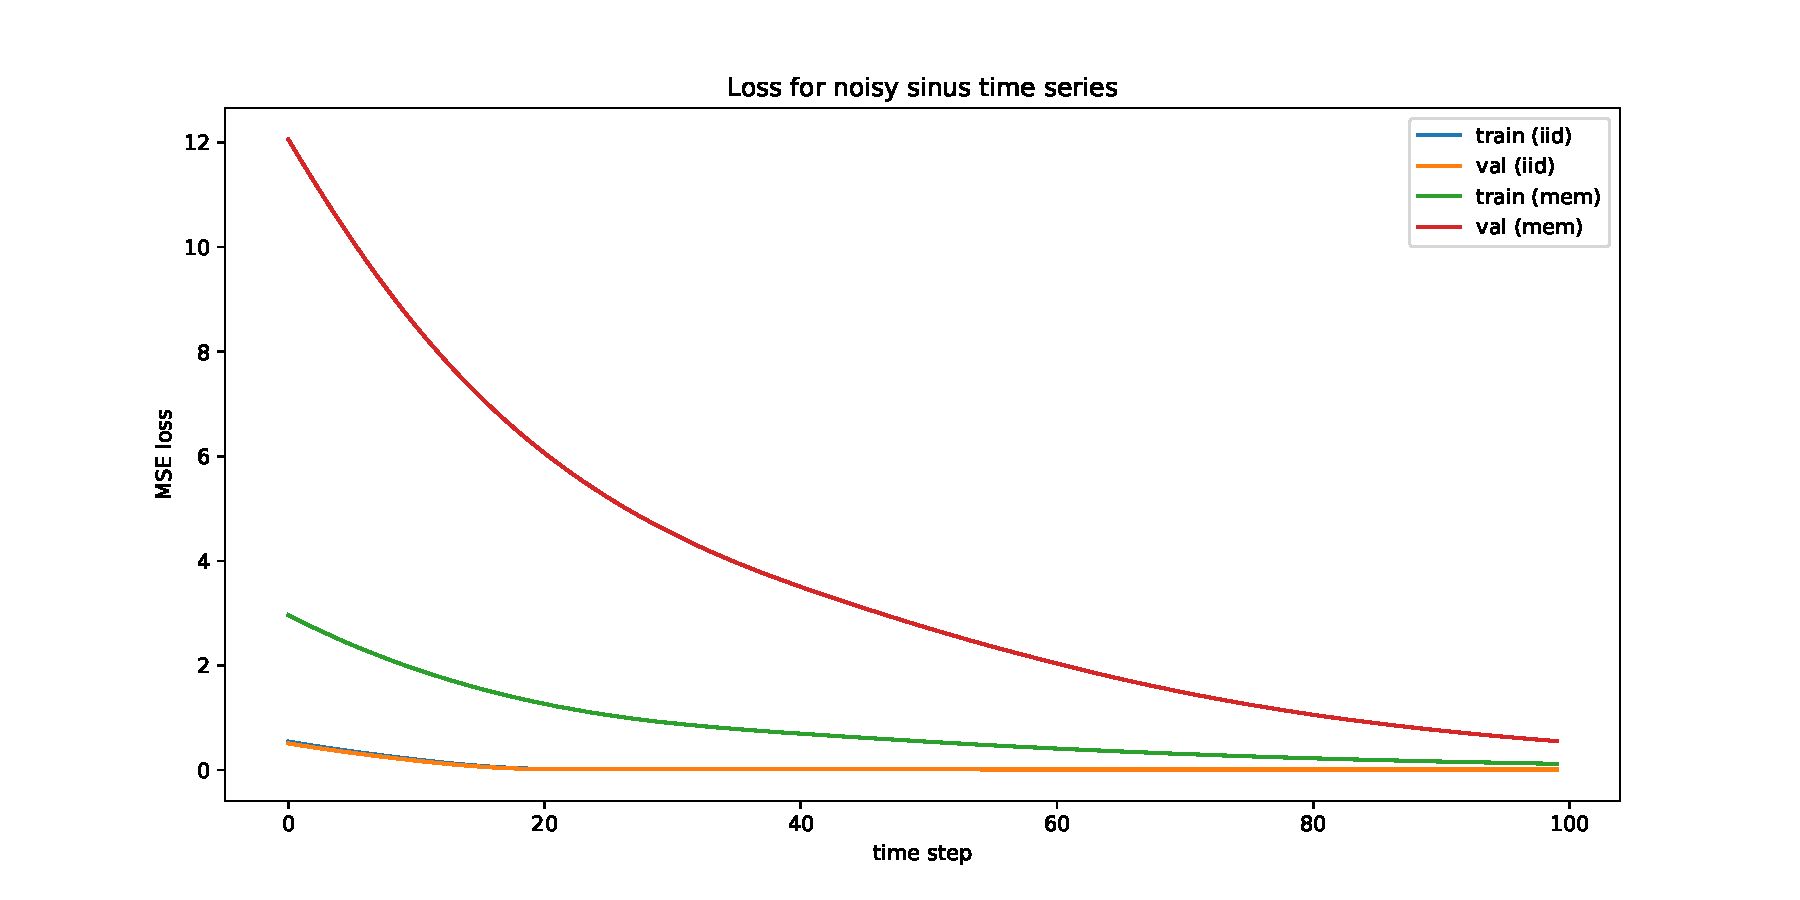
\includegraphics[width=\linewidth]{figures/plot_lstm_losscompare.pdf}
  \end{subfigure}
  \hspace{-6mm}
  \begin{subfigure}{.35\textwidth}
    \centering
    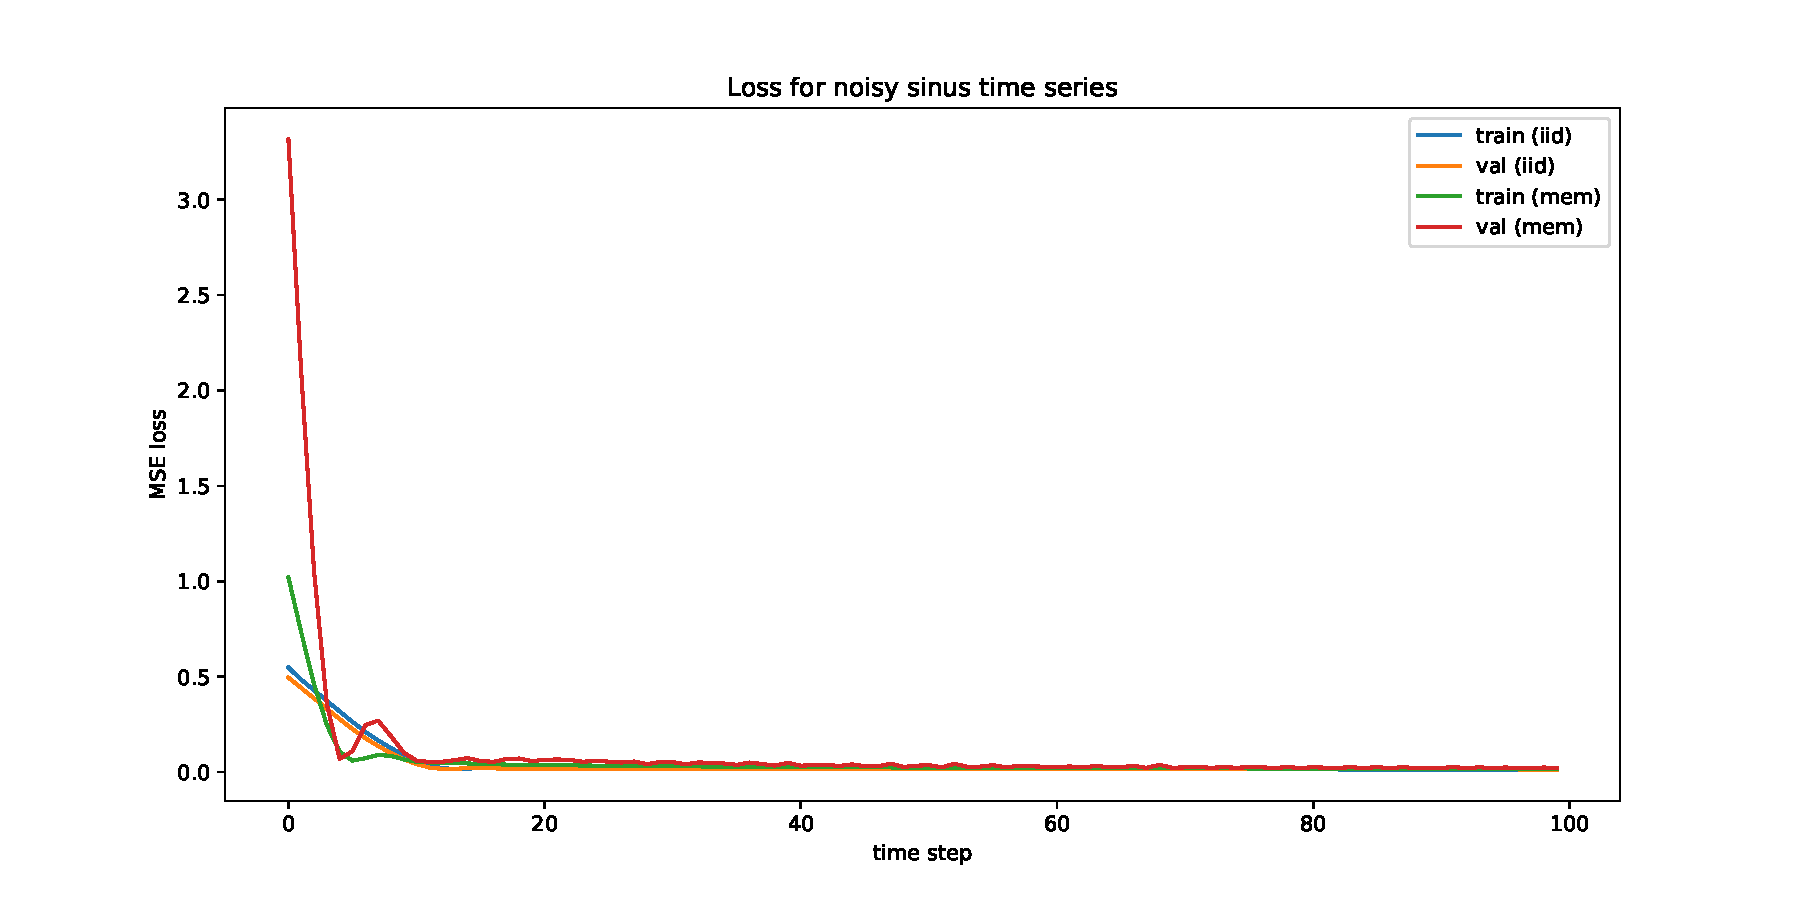
\includegraphics[width=\linewidth]{figures/plot_cnn_losscompare.pdf}
  \end{subfigure}
  \caption{MSE loss over the number of trained epochs on training and on
    validation dataset. On the left, the classical feedforward network was used.
    The middle plot shows the performance of the LSTM and the right one plots the
    loss values of the convolutional network.}
  \label{fig:noise_loss_impact}
\end{figure}

% todo: advanced feature preparation
\subsection{Mackey Glass time series forecasting}

In order to model diseases related to dynamic respiratory and hematopoietic
diseases, Mackey \textit{et al.} proposed the mackey-glass equations, a kind of
first-order nonlinear differential delay equations to model
the number of white blood cells over time \cite{mackey1977}. The solutions to
these equations given in Equation~\ref{equ:mackey}
exhibit chaotic behavior under certain conditions \cite{farmer1982}. For fixed
parameters $a = 0.2$, $b=0.1$ and $c=10$ this system has a stable fixed point
attractor for $\tau < 4.53$. With increasing delay time, the system gets less
stable. For delay times of $4.53 < \tau < 13.3$ there is a limit cycle attractor
whose period raises for $13.3 \leq \tau \leq 16.8$. For delay time
$\tau > 16.8$ the system shows chaotic behavior.

\begin{equation}
  \frac{dx}{dt} = \frac{a \cdot x(t - \tau)}{1 + x(t - \tau)^c} - b \cdot x(t)
  \label{equ:mackey}
\end{equation}

By using the Euler method to discretize the Mackey Glass time series, we can
see that the chaotic behavior gets stronger for increasing $\tau > 16.8$. In
Figure~\ref{fig:mackey_chaos}, we simulate the solution of the Mackey Glass
time series for slightly different initial conditions. It is clearly visible
that for $\tau = 17$, the time series diverges slower than for $\tau = 25$.

The first approach to predict the short-time behavior of chaotic time series
was done by Farmer \textit{et al.} who proposed a \texttt{local approximation}
technique \cite{farmer1987}. After improval of predictions using support vector
machines by Müller \textit{et al.} \cite{muller1997}, the focus in research
shifted towards artifical neural networks which enable even better predictions.
Two of the latest developments are the usage of Wavelet Networks
\cite{alexandridis2013} and particle swarm optimization \cite{caraballo2016}.

\begin{equation}
  x(t+1) = x(t) + \frac{\beta x(t - \tau)}{1 + x^{n}(t - \tau)} - \gamma x(t)
  \label{equ:mackey_euler}
\end{equation}

\begin{figure}
  \centering
  \begin{subfigure}{.5\textwidth}
    \centering
    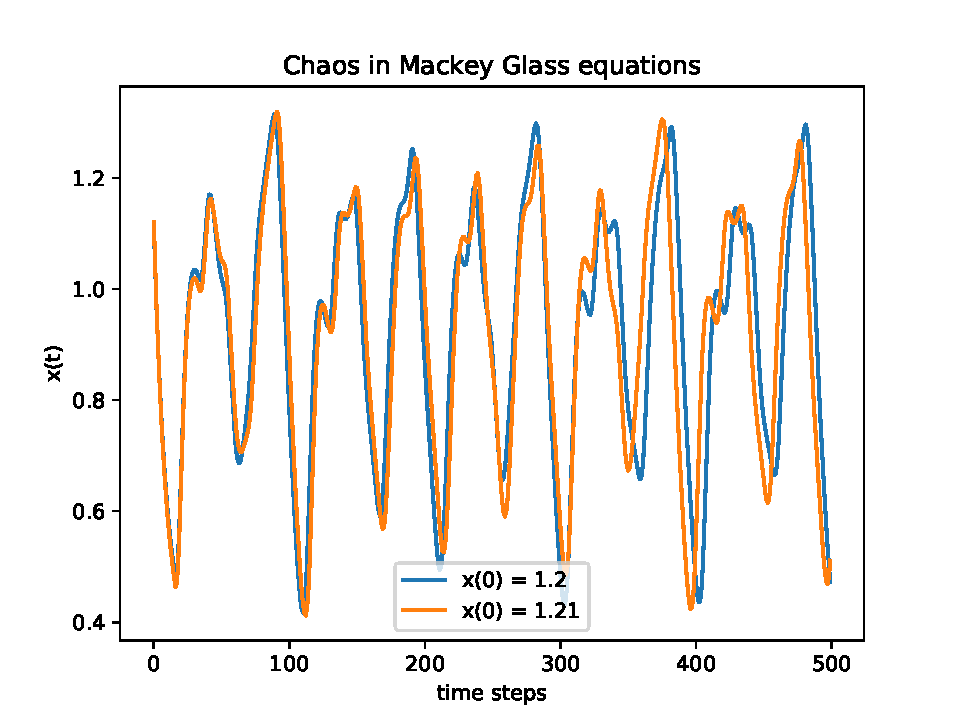
\includegraphics[width=\linewidth]{figures/mg_chaos_17.pdf}
  \end{subfigure}
  \hspace{-6mm}
  \begin{subfigure}{.5\textwidth}
    \centering
    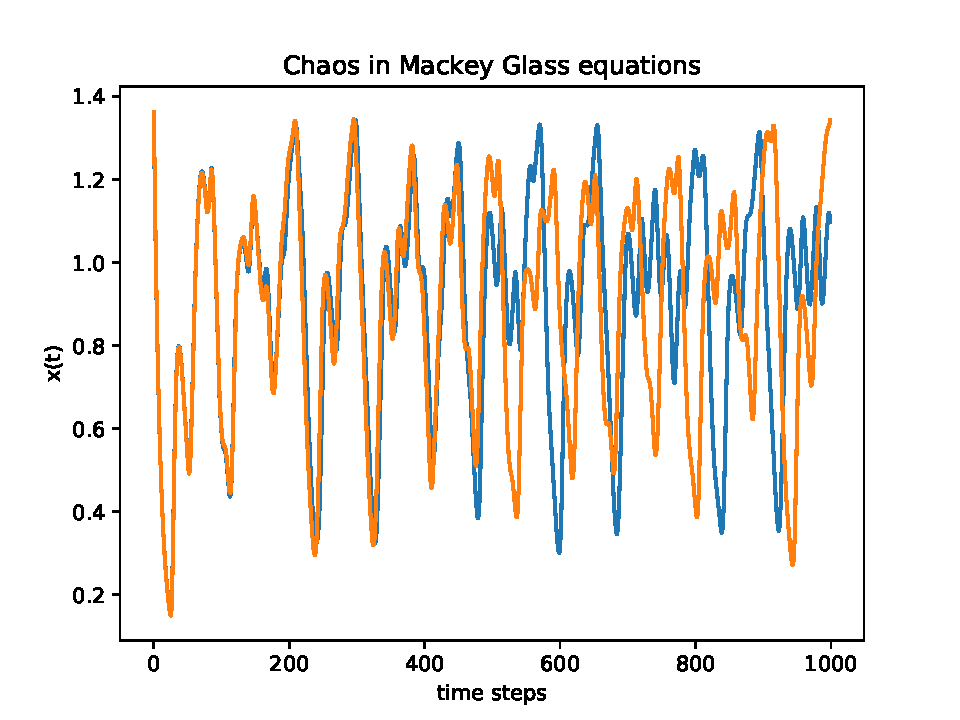
\includegraphics[width=\linewidth]{figures/mg_chaos_25.pdf}
  \end{subfigure}
  \caption{Influence of time delay parameter $\tau$ on the chaotic behavior of
    the Mackey Glass equation. The left side of the figure uses $\tau = 17$,
    the right side $\tau = 25$.}
  \label{fig:mackey_chaos}
\end{figure}

In accordance with the approach used by Caraballo \textit{et al.}
\cite{caraballo2016}, we predict $x(t+6)$ based on the information of the time
series points in $x(t)$, $x(t-6)$, $x(t-12)$, and $x(t-18)$. We investigate how
an increase in chaotic behavior impacts the prediction capability of the
different neural network architectures. The results for the feedforward neural
network are depicted in Figure~\ref{fig:mackey_cnn}. For this plot, a 2-layer
LSTM architecture was used, using 10 hidden nodes in the LSTM layer,
followed by a feedforward layer to sum up for the output value.
The first 500 time points of the time series are used for training, the 500
following points for validation. Additional 500 points are not used during the
training procedure at all and form the test set.

It can be seen that for non-chaotic solutions of the macke-glass time series the
model is able to predict precisely, and that for values of $\tau > 20$ the
chaotic behavior is strong enough to impact the prediction. We explain the low
error for $\tau = 21$ in the ability of the network to compensate for the amount
of chaos up to this point.

\begin{figure}
  \centering
  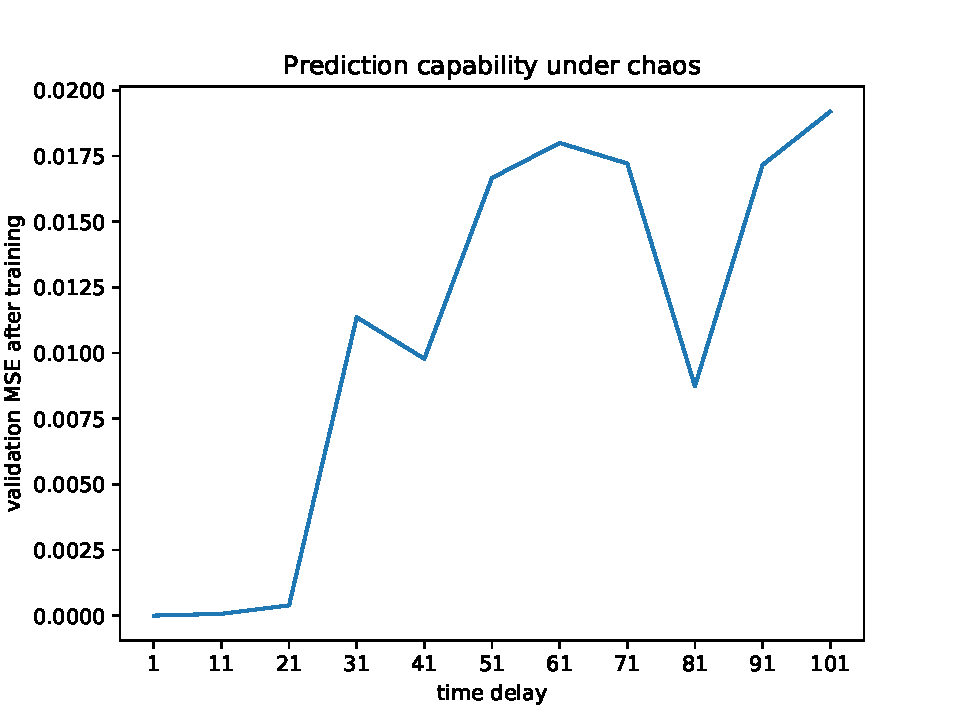
\includegraphics[width=0.6\textwidth]{figures/mackey_glass_cnn.pdf}
  \caption{Validation error of the convolutional neural network for different
    time delay values $\tau$ of the Mackey Glass equation. The error increases
    strongly for values of $\tau > 20$, indicating a strong chaotic behavior
    from this point.}
  \label{fig:mackey_cnn}
\end{figure}

In the next step, we compare our feedforward neural network and our LSTM
architecture with the results stated by Caraballo \textit{et al.}
\cite{caraballo2016} in Table~\ref{tab:mackey_results}. The results are based
on the root mean squared error (RMSE), computed in Equation~\ref{equ:rmse}.
From our considered models, the \emph{CNN} achieves the lowest RMSE value and
allows for accurate prediction, both for validation and for test data as seen
in Figure~\ref{fig:mackey_pred}. This \emph{CNN} uses three convolutional layers
with 1D convolutions, kernel size of 3, "same" padding and 8
filters each. A classical
feedforward layer without activation function is used to extract the output
value for the time series prediction.

The \emph{LSTM} employs 10 LSTM nodes, followed by a feedforward layer to sum up
the results. A variety of other layer configurations has been applied
on the problem,
but all consistently perform worse than the other neural network architectures.
We assume that the chaotic behavior of the time series confuses the \emph{LSTM}
which is trying to account for temporal dependencies between the time series
points.

\begin{figure}
  \centering
  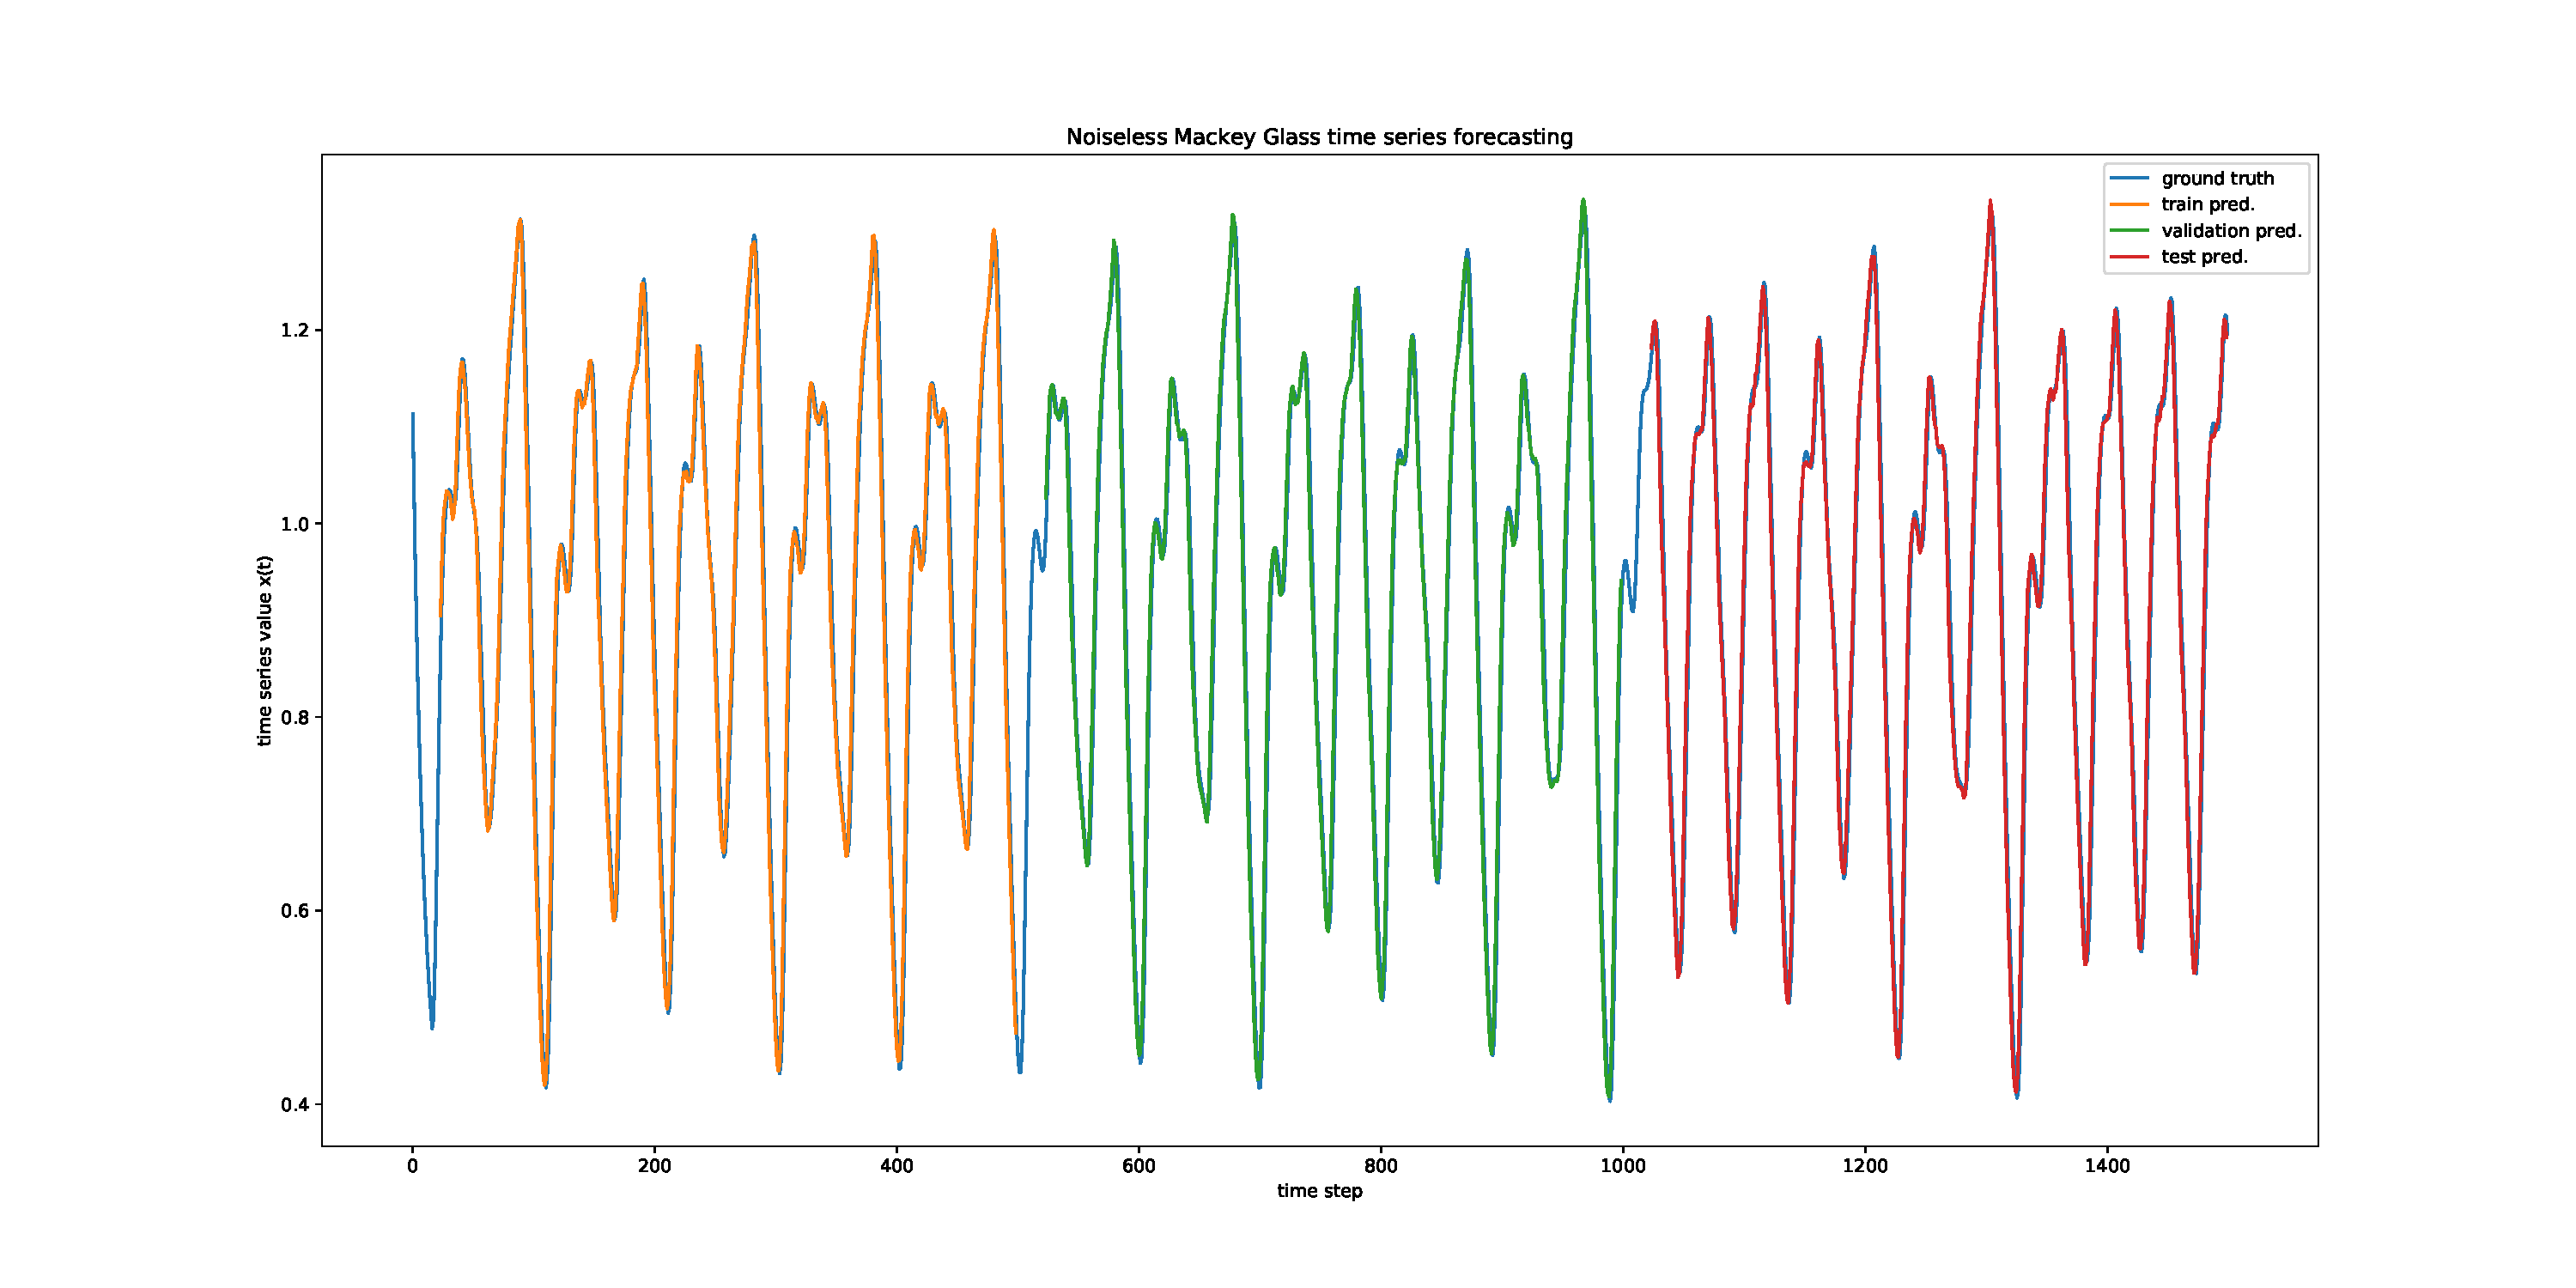
\includegraphics[width=\linewidth]{figures/mg_pred_cnn.pdf}
  \caption{The prediction of the noisefree Mackey Glass time series using a
    \emph{CNN}. The precise predictions for training, validation and testing
    points show the accurate approximation of the chaotic time series.}
  \label{fig:mackey_pred}
\end{figure}

\begin{equation}
  RMSE = \sqrt{\frac{\sum_{i=1}^n (y_i - \hat{y}_i)^2}{n}}
  \label{equ:rmse}
\end{equation}

\begin{table}
  \centering
  \begin{tabular}{c|c}
    Method                         & $RMSE_{x(t+6)}$                          \\
    \hline
    Linear model                   & 0.5503                                   \\
    Cascade correclation NN        & 0.0624                                   \\
    \textit{proposed LSTM}         & 0.0131                                   \\
    \textit{proposed MLP}          & 0.0125 (vs. 0.0262 \cite{caraballo2016}) \\
    RBFNN                          & 0.0114                                   \\
    \textit{proposed CNN}          & 0.0075                                   \\
    ANN + PSO \cite{caraballo2016} & 0.0053                                   \\
  \end{tabular}
  \caption{Mackey Glass time series forecasting results using different neural
    network architectures.}
  \label{tab:mackey_results}
\end{table}

Now we apply noise on the mackey glass time series to account for the imperfect
data characteristic to biological measurements. The results for these 
experiments are stated in Table~\ref{tab:mackey_noise}. We see that an increased
standard deviation of the added noise increases the test error, measured in 
RMSE. This applies to all neural network architectures. 

But more interestingly,
the negative effect of the noise is stronger if the noise is memorizing, i.e. if
the effect of the noise in time step $t$ impacts the time series in time step 
$t + 1$. We explain this with an increase in chaotic behavior induced by this
type of noise to the Mackey Glass time series. Since chaotic time series by 
definition deviate exponentially based on small variations in the initial
conditions, it seems logical that this divergence is increased by introducing
perturbations of the time series in every time step.

\begin{table}
  \centering
  \begin{tabular}{c|c|c|c}
    Architecture & noise type & $\sigma$ & RMSE \\
    \hline
    CNN & iid & 0.01 & 0.0196 \\
    CNN & iid & 0.1 & 0.0806 \\
    CNN & wiener & 0.01 & 0.0242 \\
    CNN & wiener & 0.1 & 0.2172 \\
    MLP & iid & 0.01 & 0.0249 \\
    MLP & iid & 0.1 & 0.0949 \\
    MLP & wiener & 0.01 & 0.0348 \\
    MLP & wiener & 0.1 & 0.2162 \\
    LSTM & iid & 0.01 & 0.0432 \\
    LSTM & iid & 0.1 & 0.0862 \\
    LSTM & wiener & 0.01 & 0.0347 \\
    LSTM & wiener & 0.1 & 0.2044 \\
  \end{tabular}
  \caption{low}
  \label{tab:mackey_noise}
\end{table}

\subsection{Biological oscillator time series forecasting}

The next section deals with time series forecasting of biological oscillators,
as described by Novak \textit{et al} \cite{novak2008}. For different aspects of
cell physiology, e.g. the DNA synthesis, this kind of oscillators can be
observed. Novak \textit{et al.} show that oscillations in simple ODEs can be
produced by incorporating an explicit time delay \cite{novak2008}, similar to
the Mackey Glass equations \cite{mackey1977}.

Recently, Strömstedt \textit{et al.} analyzed the capability of neural network
architectures to model stochastic time series \cite{stroemstedt2018} at the
example of time series produced according to the characteristics of Novak
\textit{et al} \cite{novak2008}. In this section, we reproduce their results for
the LSTM architecture and state fundamental limits for neural networks to
approximate stochastic time series.

The time series data is generated using \texttt{gillespy} \cite{abel2016}.
Using this framework, a simple stochastic reaction system with 2 states is
set up. One protein $X$ is produced more the less of the other protein $Y$
exists. $X$ and $Y$ are both continuously reduced but $Y$ gets reduced stronger
for smaller values of $Y$. A set of 7 parameters is used to parametrize the
system.

The motivation for using neural netowrks to generate time series is the
computational expensiveness of analytical solutions like the Gillespie
algorithm \cite{gillespie1977}. On experiments on our hardware
(see Table~\ref{tab:hardware} for details)
we need more than 6 seconds to simulate the biological oscillator with two
states. This makes grid search approaches on the large number of parameter
combinations intractable. Using the 2-layer LSTM approach, predictions for
short time series can be done in less than $0.2$ seconds on our hardware.

The goal here is to train a LSTM based
model to convert a set of input parameters into a time series. The first
LSTM layer
takes 7 input values and transforms them into $n$ sequences of 7 values, with
$n$ being the desired length of the output sequence. The second LSTM layer
takes this result and converts it to a sequence of length $n$.

The analysis of the resulting time series as depicted in
Figure~\ref{fig:nn_limitation} shows the general limitation of using a
deterministic neural network for predicting a stochastic time series. For one
possible of parameters for the biological oscillator, the analytical solution
was computed under $100$ (stochastic) trajectories. After that, the network was
trained to predict the time series based on the (unchanged) parameters. We see
that the short-term predictions are accurate and have the same magnitude as the
ground truth signal -- but the more time steps are simulated, the larger is the
difference between the ground truth trajectories due to stochasticity. In other
words, the neural network predicts the mean of the signals and the amplitude
decreases due to the increasing variance of the signal over time.
It should be noted that the trends in the time series are still
recognized, just with a smaller amplitude.

\begin{table}
  \centering
  \begin{tabular}{cc}
    Processor & Intel(R) Core i5-7200U CPU @ 2.50GHz \\
    RAM       & 7859 MB                              \\
  \end{tabular}
  \caption{Hardware configuration used in experiments.}
  \label{tab:hardware}
\end{table}

\begin{figure}
  \centering
  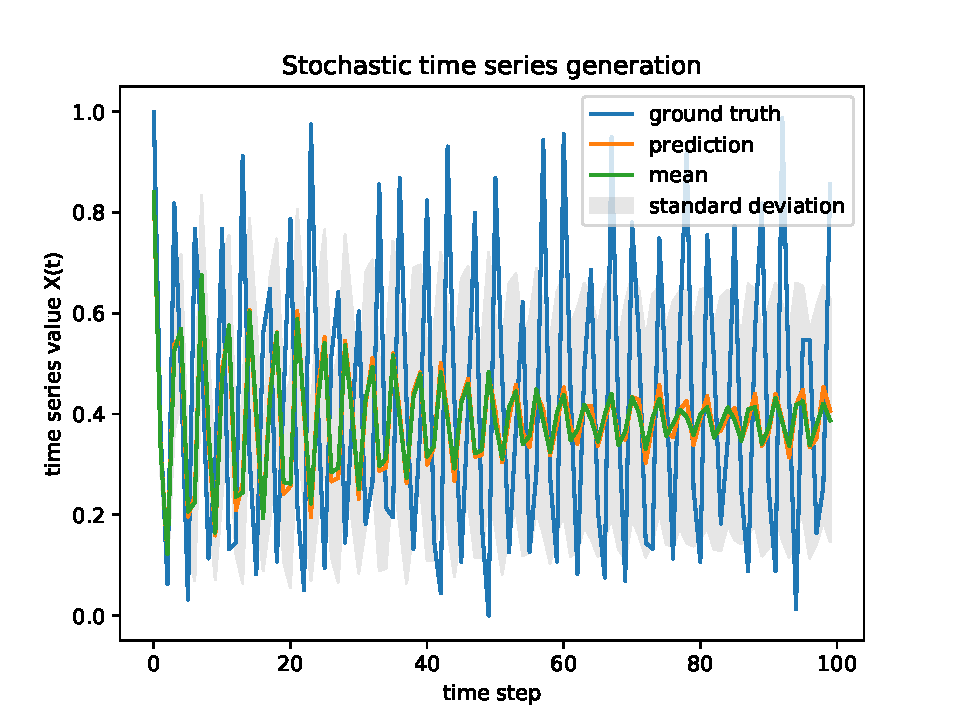
\includegraphics[width=\textwidth]{figures/nn_limitation.pdf}
  \caption{Prediction of stochastic time series using deterministic
    \textbf{LSTM} network. Sampled ground truth data are unseen for the network.
    Mean computed on all stochastic trajectories.}
  \label{fig:nn_limitation}
\end{figure}

\section{Conclusion}

In this report, we investigate how chaotic time series can be approximated
using neural networks. It is possible to improve the forecasting results by
advanced architectures. Especially the convolutional neural networks
outperform the feedforward neural network with one hidden layer,
although theoretically all classes are capable of approximating any continuous
function. We assumed that the hierarchical features in time series can be
captured better using a \emph{LSTM} by capturing time dependencies or a
\emph{CNN} for extracting hierarchical features, but the results indicate that
the convolutional neural networks also show superior performance in this area.
Unfortunately, it is also shown that neural networks can only be used to
generate stochastic time series in a limited way. Since the prediction operation
is deterministic, the possibility of predicting the stochastic time series
declines with the length of the prediction. Only the general trends can be seen
from the neural network, the amplitude declines below the level of the
original time series.

\bibliographystyle{alpha}
\bibliography{report}

\end{document}